\chapter{Magnetic Resonance Imaging}
\label{chapterlabel2}

This section provides the necessary mathematical background for understanding the magnetic resonance imaging process. It starts with describing the NMR (nuclear magnetic resonance) phenomena which are at the heart of magnetic resonance imaging, continues with the basic concepts behind image formation and ends with a description of parallel imaging, the main focus of this thesis.

%%%%%%%%%%%%%%%%%%%%%%%%%%
\section{NMR Physics}
Magnetic resonance imaging (MRI) is a non-invasive imaging technique that is based on the physical phenomena of atomic nuclei (protons) responding and interacting with external magnetic fields. The key participant in the process of constructing MR images is the hydrogen proton, the most abundant element in our bodies. In fact, other species of protons can also be used, but in this thesis the main focus is on the hydrogen proton. For the most part, an MRI experiment is made up of two steps. First, a series of magnetic fields are used to manipulate the proton 'spin' orientation in order to create a net magnetization arising from the collective spins. Second, this net magnetization is manipulated with radio frequency magnetic fields in order to be measured using a coil detector. That being said, in this subsection the focus is on the underlying physics of magnetic resonance imaging, starting from the behaviour of a single magnetic moment placed in a static magnetic field and ending with the principles of signal detection.

%%%%%%%%%%%%%
\subsection{Classical Response of a Single Nucleus to a Magnetic Field}
In magnetic resonance imaging the key participator is the magnetic moment of the proton. In this subsection the fundamental interaction of a proton when placed in a static magnetic field is described.

Following the work of Stern and Gerlach in the early 1920's, 
a fundamental property of an odd numbered atomic nucleus was inferred from experiment. 
This property is called \textit{angular momentum $\vec{J}$} (or \textit{spin}) and it gives rise, from a classical perspective, to a small \textit{magnetic moment} $\vec{\mu}$. 
The relationship between the two properties is found from experiment:

\begin{equation} \label{eq:21}
    \vec{\mu} = \gamma \vec{J}
\end{equation}

where $\gamma$ is called the \textit{gyromagnetic ratio} and it is a particle dependent constant. For hydrogen nuclei, this quantity is found to be:

\begin{equation} \label{eq:22}
    \gamma_{H} = 2.675 \times 10^8 \text{  } rad/s/T
\end{equation}

or the 'gamma-bar' quantity:

\begin{equation} \label{eq:23}
    \text{\sout{$\gamma$}}_H \equiv \frac{\gamma}{2 \pi} = 42.58 \text{  } MHz/T
\end{equation}
where T is Tesla, the unit for magnetic field strength, and it is the equivalent of $10,000$ Gauss \cite{Haacke1999}.

In addition, when placing the spin in an external magnetic field $\vec{B}$, it will experience a torque $\vec{N}$ that will align the magnetic moment $\vec{\mu}$ along the direction of the field according to
\begin{equation} \label{eq:24}
    \vec{N} = \vec{\mu} \times \vec{B}
\end{equation}
Furthermore, knowing that a nonzero net torque on a loop implies that the total angular momentum $\vec{J}$ will change with:

\begin{equation} \label{eq:25}
    \frac{d\vec{J}}{dt} = \vec{N}
\end{equation}

and taking into account equations \ref{eq:21} and \ref{eq:24}, we find the following:

\begin{equation} \label{eq:26}
    \frac{d\vec{\mu}}{dt} = \gamma \vec{\mu} \times \vec{B}
\end{equation}
which is the fundamental equation of motion for a single spin in a magnetic field.

Furthermore, by forming a scalar (dot) product of both sides of equation \ref{eq:26} we get:

\begin{flalign*}
	\frac{d\vec{\mu}}{dt} \cdot \vec{\mu} + \vec{\mu} \cdot
	     \frac{d\vec{\mu}}{dt} &= 0  \Rightarrow \\
	\frac{d(\vec{\mu} \cdot \vec{\mu})}{dt} &= 0  \Rightarrow \\
	\frac{d\mu^2}{dt} &= 0 \Rightarrow \\
	\frac{d \mu}{dt} \, \mu + \mu \, \frac{d \mu}{dt} &= 0 \Rightarrow \\
	2 \, \mu \, \frac{d \mu}{dt} &= 0 \Rightarrow \\
	\frac{d \mu}{dt} &= 0
\end{flalign*}

which shows that the magnitude of the magnetic moment does not change with time. On the other hand, the direction of the magnetic moment does change with time, the cross product between $\vec{\mu}$ and $\vec{B}$ 'pushing' the tip of the magnetic moment vector in a clockwise precession. This behaviour is shown in Figure~\ref{fig:21} where the angular frequency of precession is found with the following deduction: \\

We know that:
\begin{equation} \label{eq:27}
    \lvert d\vec{\mu} \rvert = 
        \lvert \vec{\mu} \rvert sin \theta \lvert d \phi \rvert 
\end{equation}

But we also know that:
\begin{equation} \label{eq:28}
    \lvert d\vec{\mu} \rvert = 
        \gamma \lvert \vec{\mu} \times \vec{B} \rvert dt = 
        \gamma \, \mu \, B \, sin \theta \, dt 
\end{equation}

Therefore, from equations \ref{eq:27} and \ref{eq:28} above we get:
\begin{equation} \label{eq:29}
    \lvert d\phi \rvert = \gamma \, B \, \lvert dt \rvert
\end{equation}

which brings us to the well-known \textit{Larmor precession} formula given below:
\begin{equation} \label{eq:210}
    \omega \equiv \lvert \frac{d\phi}{dt} \rvert = \gamma B
\end{equation}

This equation is at the heart of MR imaging as it relates the strength of the magnetic field and the frequency of the spins' precession. 

\begin{figure}[ht]
    \centering
    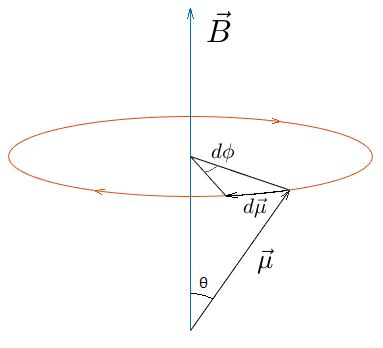
\includegraphics[width=0.7\textwidth,keepaspectratio]{precession}
    \caption{Clockwise precession of a proton's spin about a magnetic field}
    \label{fig:21}
\end{figure}

%%%%%%%%%%%%%
\subsection{Rotating reference frames and resonance}
So far we have seen how a single spin behaves when placed in a static magnetic field. Next, our focus shifts to the magnetic moment's behaviour when the combined effect of two perpendicular fields is present. This is an important step to consider as it is one of the requirements when generating a detectable signal. Therefore, in this subsection the mathematics behind rotating reference frames and harmonic fields is presented. Also, it is shown that the magnetic moment can be effectively rotated away from the static field's direction by using an RF field that matches the Larmor frequency.

\begin{figure}[ht]
    \centering
    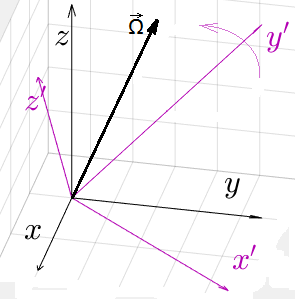
\includegraphics[width=0.7\textwidth,keepaspectratio]{primedframe}
    \caption{The primed reference frame rotating according to the angular velocity vector $\vec{\Omega}$}
    \label{fig:22}
\end{figure}

To start with, let us consider two reference frames, a fixed (unprimed) and a rotating one (primed), such that the latter is rotating about an arbitrary axis with respect to the static one (see Figure~\ref{fig:22}). The rotation is defined by a rotational angular velocity vector $\vec{\Omega}$ and any vector $\vec{V}$ at rest in the rotating frame will have its time rate of change equal to:

\begin{equation}
    \frac{d\vec{V}}{dt} = \vec{\Omega} \times \vec{V}    
\end{equation}

Next, let's consider an arbitrary vector function $\vec{C}(t)$ defined by as $\vec{V}(t) = V_x(t) \hat{x} + V_y(t) \hat{y} + V_z(t) \hat{z}$ in the fixed coordinate system. Alternatively, it can also be expressed in terms of the primed reference frame and it will take the following form: $\vec{V}(t) = V_{x'}(t) \hat{x}(t) + V_{y'}(t) \hat{y}(t) + V_{z'}(t) \hat{z}(t)$. As the two representations refer to the same vector, taking the time derivative of $\vec{V}(t)$ in both forms should yield the same answer, i.e.,

\begin{flalign*}
	\frac{dV_x}{dt}\hat{x} + \frac{dV_y}{dt}\hat{y} + \frac{dV_z}{dt}\hat{z} 
	\, = \, & \frac{dV_{x'}}{dt} \hat{x}'(t) + \frac{dV_{y'}}{dt} \hat{y}'(t) + \frac{dV_{z'}}{dt} \hat{z}'(t) + \\
	& V_{x'}\frac{d\hat{x}'(t)}{dt} + V_{y'}\frac{d\hat{y}'(t)}{dt} + 
	        V_{z'}\frac{d\hat{z}'(t)}{dt}
\end{flalign*}

We know that any vector at rest in the primed coordinate system will have its time derivative with respect to the unprimed system defined as the cross product between the angular velocity vector and itself. As a result, the time derivatives of the unit vectors from the equation above can be written as: $\frac{d\hat{x}'}{dt} = \vec{\Omega} \times \hat{x}'$, $\frac{d\hat{y}'}{dt} = \vec{\Omega} \times \hat{y}'$ and $\frac{d\hat{z}'}{dt} = \vec{\Omega} \times \hat{z}'$.

From here we can write the compact form of our equation as such:

\begin{equation} \label{eq:212}
    \frac{d\vec{V}}{dt} = (\frac{d\vec{V}}{dt})' + \vec{\Omega} \times \vec{V}
\end{equation}

Replacing our arbitrary vector $\vec{V}(t)$ with the magnetic moment $\vec{\mu}$ we get:
\begin{equation} \label{eq:213}
    \frac{d\vec{\mu}}{dt} = (\frac{d\vec{\mu}}{dt})' + \vec{\Omega} \times \vec{\mu}
\end{equation}

From equations \ref{eq:26} and \ref{eq:213} we can write:

\begin{flalign*}
	 (\frac{d\vec{\mu}}{dt})' &= \gamma \vec{\mu} \times \vec{B} - \vec{\Omega} \times \vec{\mu} \Rightarrow \\
	(\frac{d\vec{\mu}}{dt})' &= \gamma \vec{\mu} \times \vec{B} + \vec{\mu} \times \vec{\Omega} \Rightarrow \\
	(\frac{d\vec{\mu}}{dt})' &= \gamma \vec{\mu} \times (\vec{B} + \frac{\vec{\Omega}}{\gamma})
\end{flalign*}

which yields 

\begin{equation} \label{eq:214}
    (\frac{d\vec{\mu}}{dt})' = \gamma \vec{\mu} \times \vec{B}_{eff}
\end{equation}

and therefore shows that in the rotating reference frame the precession motion of the magnetic moment vector can be described according to an 'effective magnetic field' \cite{Haacke1999}. This is a key concept in MRI as it is the basis of magnetic moment analysis in general.

Next, we need to show how to construct this magnetic field so that we can most effectively 'tip' the magnetic moment vector in the transverse plane. It is clear from equation \ref{eq:214} that $\vec{B}_{eff}$ has to have both $x$ and $y$ components in order to move the magnetic moment away from the $z$ axis. For this we can combine our static field $\vec{B}_0 = B_0 \hat{z}$ with a circularly polarised 
rf field $\vec{B}_1^{cir} = B_1(\hat{x} \, cos \omega t - \hat{y} \, sin \omega t) = B_1 \hat{x}'$. By substituting in equation \ref{eq:214} we get:

\begin{equation} \label{eq:215}
    (\frac{d\vec{\mu}}{dt})' = \vec{\mu} \times [\hat{z}'(\omega_0 - \omega) + \hat{x}' \omega_1] = \gamma \vec{\mu} \times \vec{B}_{eff}
\end{equation}

where $\omega_0 = \gamma B_0$ is the Larmor frequency, $\omega$ is the rf field's laboratory frequency and $\omega_1 = \gamma B_1$ is the spin precession frequency generated by $\vec{B}_1^{cir}$.

It is clear from the above equation that an effective 'tipping' around the $\hat{x}'$ axis will happen when the applied rf field's frequency is equal to the Larmor frequency. This leads to the equation of motion of the magnetic moment in the rotating reference frame:

\begin{equation} \label{eq:216}
    (\frac{d\vec{\mu}}{dt})' = \omega_1 \vec{\mu} \times \hat{x}'
\end{equation}

while the condition that accomplishes this:

\begin{equation} \label{eq:217}
    \omega = \omega_0    
\end{equation}

is called the \textit{on-resonance condition}.

In fact, this rotation can be controlled by choosing the amount of time the on-resonance rf field is applied. For a finite amount of time $\tau$, the angle of rotation, called the \textit{flip angle}, can be calculated with the following formula:

\begin{equation} \label{eq:218}
    \Delta \theta = \gamma B_1 \tau
\end{equation}

For example, for a $90^o$ flip angle, the $B_1$ field should have a magnitude of $5.9 \, \mu T$ and be applied for $1.0 \, ms$ for hydrogen protons \cite{Haacke1999}.


%%%%%%%%%%%%%
\subsection{Magnetization, Relaxation and the Bloch Equation}
In the previous subsections, the focus was on a single proton's spin. 
%Also, rotating reference frames and the resonance condition for effectively tipping the magnetic moment were discussed. 
In this subsection, a collection of spins is considered and the interactions with their environment is described. The focus is on the phenomenological Bloch equation that models the relaxation phenomena by means of decay times.

In MRI, as the objects we are imaging are on a macroscopic scale, the next logical step is to consider collections of spins. Therefore, a vector quantity called the \textit{magnetization vector} $\vec{M}(\vec{r},t)$ is now introduced and it is defined as the local magnetic moment per unit volume. Considering a volume $V$ such that all spins residing inside it experience the same external magnetic field, the magnetization is defined as:

\begin{equation} \label{eq:219}
    \vec{M} = \frac{1}{V} \sum_{i \in \text{protons in V}} \vec{\mu}_i
\end{equation}

This set of spins is called an \textit{isochromat} and, ideally, it contains spins which have the same phase. Under these circumstances, extending equation \ref{eq:26} to the volume $V$ we arrive at:

\begin{equation} \label{eq:220}
    \frac{1}{V} \sum_i \frac{d\vec{\mu}_i}{dt} = \frac{\gamma}{V} \sum_i \vec{\mu}_i \times \vec{B}
\end{equation}

which, together with equation \ref{eq:219} yields:

\begin{equation} \label{eq:221}
    \frac{d\vec{M}}{dt} = \gamma \vec{M} \times \vec{B}
\end{equation}
for non-interacting protons.

Decomposing this magnetization vector into parallel and perpendicular components ($\vec{M}_{\parallel} = M_z \hat{z}$ and $\vec{M}_{\perp} = M_x \hat{x} + M_y \hat{y}$) while considering $\vec{B} = B_0 \, \hat{z}$, we arrive at the following two equations:

\begin{equation} \label{eq:222}
    \frac{dM_z}{dt} = 0
\end{equation}

\begin{equation} \label{eq:223}
    \frac{d\vec{M}_{\perp}}{dt} = \gamma \vec{M}_{\perp} \times \vec{B}
\end{equation}

both for non-interacting protons.

It follows now that our next discussion turns to interacting protons. This leads to additional terms in the previous equations which are due to the energy exchange between the spins and their environment, and between themselves. These terms describe different relaxation phenomena because the magnetization vector does not have a fixed magnitude, since it is the sum of individual proton spins. 

At thermal equilibrium and when exposed to a constant, static magnetic field $\vec{B} = B_0 \, \hat{z}$, the magnetization vector is:

\begin{equation} \label{eq:224}
    \vec{M} = M_0 \, \hat{z}
\end{equation}

where $M_0$ is found from quantum statistics to be:

\begin{equation} \label{eq:225}
    M_0 = \frac{\gamma^2 \text{\sout{$h$}}^2 \, B_0 \, \rho}{4 \, K \, T}
\end{equation}

where \sout{$h$} is the reduced Planck constant $h$ ($6.626 \times 10^{-34} J$) or \textit{h-bar} and is equal to $\frac{h}{2 \pi}$, $\rho$ is the number of spins per unit volume (spin density), $K$ is the Boltzmann constant ($1.38 \times 10^{-23} J \, K^{-1}$) and $T$ is the absolute temperature of the system in Kelvin \cite{Haacke1999}. As can be seen from this equation, the only controllable parameter is the external magnetic field's strength, or $B_0$, which in MRI scanners can range between 0.2 to 9 Tesla. 

Now, if the external magnetic field experiences any disturbance, the spin system will be taken out of its initial thermal equilibrium state. However, according to the laws of thermodynamics, the system will return to that state if enough time is given. In MRI, this process can be characterized by two independent relaxation phenomena which are summarized below:

\begin{enumerate}
    \item \textbf{The Spin-Lattice Interaction} which causes the relaxation of the \textit{longitudinal} component of the magnetization vector.
    
    \item \textbf{The Spin-Spin Interaction} which causes the disappearance of the \textit{transverse} component of the magnetization vector.
\end{enumerate}

Under these circumstances, the equations presented above for non-interacting protons have to be changed to accommodate the spin's interaction with their environment. First, the spin-lattice interaction introduces a constant growth rate called $T_1$ which is empirically determined and changes equation \ref{eq:222} to:

\begin{equation} \label{eq:226}
    \frac{dM_z}{dt} = \frac{1}{T_1} (M_0 - M_z) \, \text{ (for } \vec{B}_0 \parallel \hat{z} \text{)}
\end{equation}

with the solution:

\begin{equation} \label{eq:227}
    M_z(t) = M_z(0) e^{-t/T_1} + M_0(1-e^{-t/T_1}) \, \text{ (for } \vec{B}_0 \parallel \hat{z} \text{)}
\end{equation}

Second, the spin-spin interaction introduces a decay rate called $T_2$ which is also empirically determined and which changes equation \ref{eq:223} to:

\begin{equation} \label{eq:228}
    \frac{d\vec{M}_{\perp}}{dt} = \gamma \vec{M}_{\perp} \times \vec{B} - \frac{1}{T_2} \vec{M}_{\perp}
\end{equation}

or 

\begin{equation} \label{eq:229}
    (\frac{d\vec{M}_{\perp}}{dt})' = - \frac{1}{T_2} \vec{M}_{\perp} \, \text{ (in the rotating frame)} 
\end{equation}

with the solution:

\begin{equation} \label{eq:230}
    \vec{M}_{\perp}(t) = \vec{M}_{\perp}(0) e^{-t/T_2} \, \text{ (in the rotating frame)}
\end{equation}
The two solutions are shown in Figure \ref{fig:relax}.

\begin{figure}[ht]
    \centering
    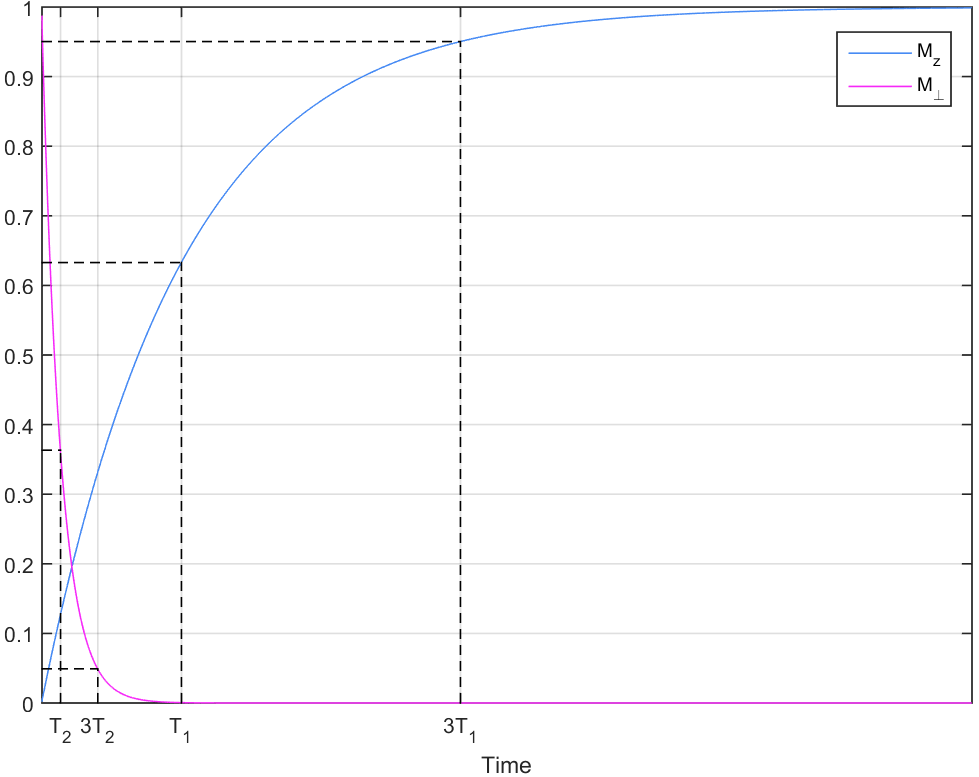
\includegraphics[width=1\textwidth,keepaspectratio]{MzMt}
    \caption{The regrowth of the longitudinal magnetization from $0$ to its initial value $M_z$ and the decay of the transverse magnetization from an initial value $M_{\perp}(0)$ to $0$} 
    \label{fig:relax}
\end{figure}

% \begin{figure}
%     \centering
    
%     \begin{subfigure}[b]{0.48\textwidth}
%         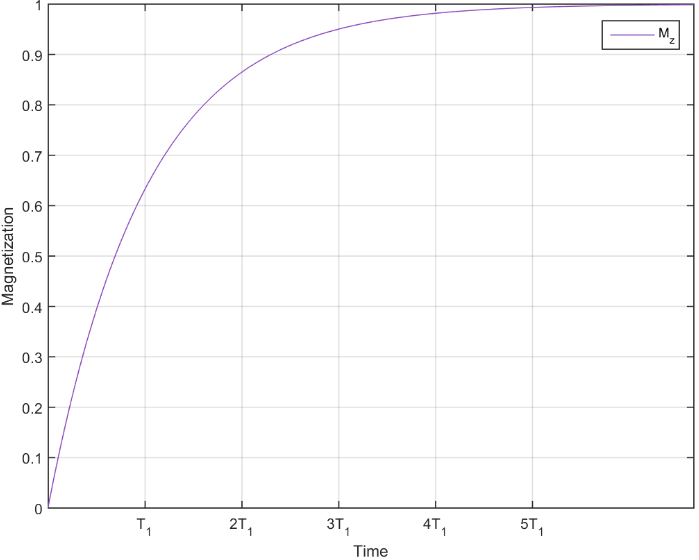
\includegraphics[width=\textwidth]{Mpara}
%         \caption{The regrowth of the longitudinal magnetization from $0$ to its initial value $M_z$}
%         \label{fig:Mpara}
%     \end{subfigure}
%     ~ %add desired spacing between images, e. g. ~, \quad, \qquad, \hfill etc. 
%       %(or a blank line to force the subfigure onto a new line)
%     \begin{subfigure}[b]{0.48\textwidth}
%         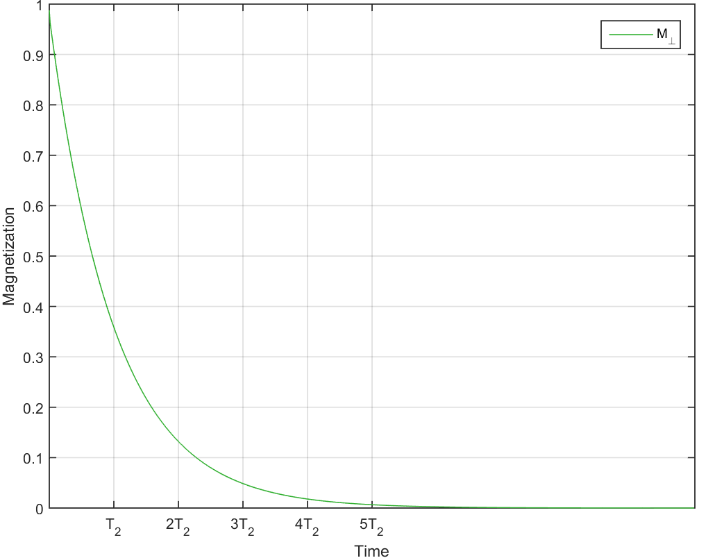
\includegraphics[width=\textwidth]{Mperp}
%         \caption{The decay of the transverse magnetization from an initial value $M_{\perp}(0)$ to $0$}
%         \label{fig:Mprep}
%     \end{subfigure}
    
    
%     \caption{TODO: Write caption text AND Label y axis with Mz(0) Mtr(0) and so on. See fig 4.1 book} 
%     \label{fig:relax}
% \end{figure}

Actually, the transverse relaxation happens at a higher rate because of additional field inhomogeneities which cause the spins to dephase faster. This is characterised by a separate decay time called $T_2'$. We can therefore define the total relaxation rate $R_2^*$ as the sum between the internal ($R_2$) and external ($R_2'$) relaxation rates: $R_2^* = R_2 + R_2'$. This yields the following relation between the relaxation times:

\begin{equation} \label{eq:231}
    \frac{1}{T_2^*} = \frac{1}{T_2} + \frac{1}{T_2'}
\end{equation}

It is noteworthy to mention that the loss of phase due to external field inhomogeneities can be recovered by means of an \textit{echo} which can be achieved under certain circumstances, while the intrinsic $T_2$ losses are not recoverable. 

It follows that an equation which combines both types of processes is defined. This one vector equation is called \textit{the Bloch equation} and is presented below:
\begin{equation} \label{eq:232}
    \frac{d\vec{M}}{dt} = \gamma \vec{M} \times \vec{B} + \frac{1}{T_1} (M_0 - M_z) \hat{z} - \frac{1}{T_2} \vec{M}_{\perp}
\end{equation} 
which, for $\vec{B} = B_0 \hat{z}$, has the following solutions:
\begin{equation} \label{eq:233}
    \frac{dM_z}{dt} = \frac{M_0 - M_z}{T_1}
\end{equation}
\begin{equation} \label{eq:234}
    \frac{dM_x}{dt} = \omega_0 M_y - \frac{M_x}{T_2}
\end{equation}
\begin{equation} \label{eq:235}
    \frac{dM_x}{dt} = -\omega_0 M_x - \frac{M_y}{T_2}
\end{equation}
where $\omega_0 = \gamma B_0$.

\begin{figure}[ht]
    \centering
    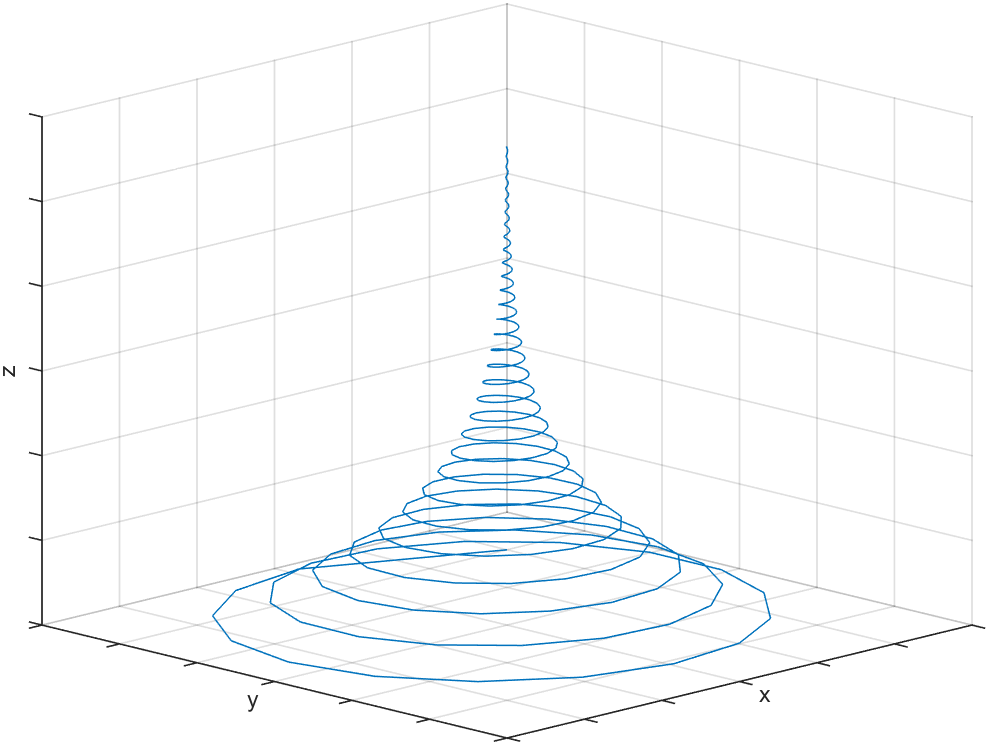
\includegraphics[width=1\textwidth,keepaspectratio]{spiral}
    \caption{The trajectory of the tip of the magnetization vector showing at the same time the regrowth and the decay of its components.}
    \label{fig:spiral}
\end{figure}

Furthermore, the three differential equations presented above have the following solutions in \textit{Cartesian representation}:
\begin{equation} \label{eq:236}
    M_x(t) = e^{-t/T_2} (M_x(0) \, cos \, \omega_0 t + M_y(0) \, sin \, \omega_0 t)
\end{equation}
\begin{equation} \label{eq:237}
    M_y(t) = e^{-t/T_2} (M_y(0) \, cos \, \omega_0 t - M_x(0) \, sin \, \omega_0 t)
\end{equation}
\begin{equation} \label{eq:238}
    M_z(t) = M_z(0) e^{-t/T_1} + M_0 (1 - e^{-t/T_1})
\end{equation}
with the following steady-state solutions: $M_x(\infty) = M_y(\infty) = 0$ and $M_z(\infty) = M_0$.

A graphical representation of the magnetization vector components evolution throughout time for a white matter tissue sample with $T_1 = 600 \, ms$ and $T_2 = 80 \, ms$, placed in a constant magnetic field of strength $B = 7 \, T$ can be found in Figure~\ref{fig:MxMyMz}, while the three dimensional representation of how the magnetization vector reaches its equilibrium state can be seen in Figure~\ref{fig:spiral}.

\begin{figure}[ht]
    \centering
    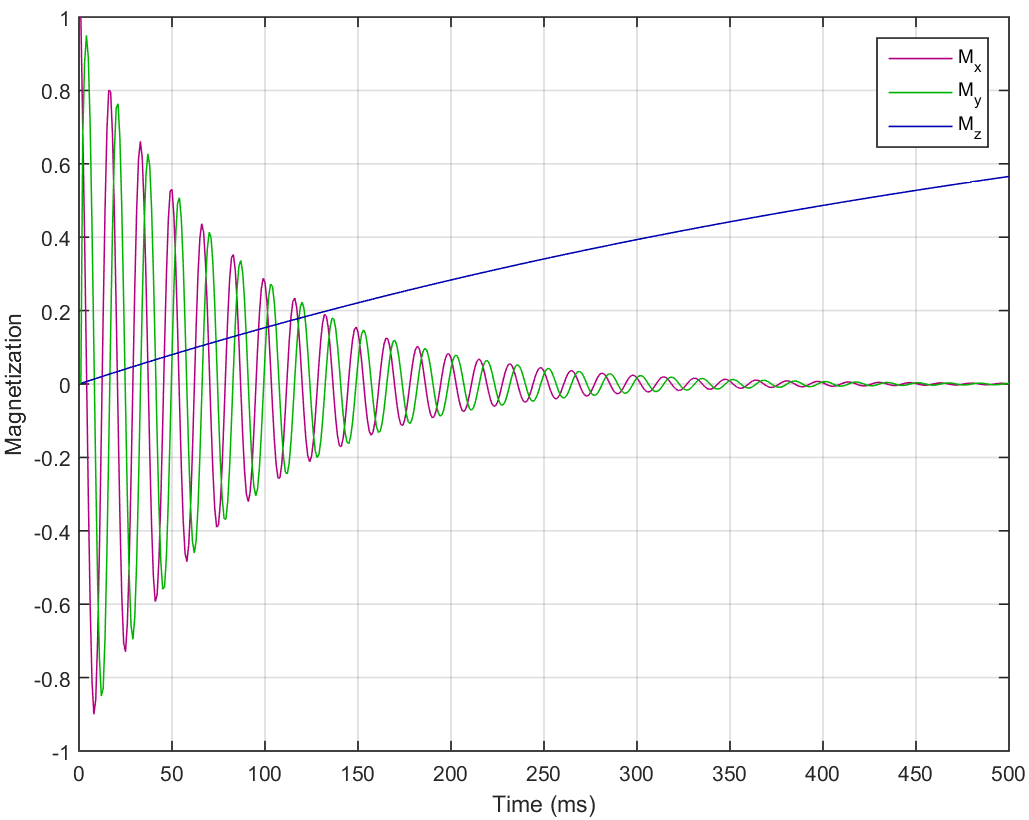
\includegraphics[width=1\textwidth,keepaspectratio]{MxMyMz}
    \caption{The regrowth of the longitudinal $M_z$ component of the magnetization vector from $0$ to its initial value $M_0$ shown in blue and the decay of both transverse components $M_x$ and $M_y$ from an initial value to 0 shown in purple and green. $M_0$ is considered to be equal to $1$ for illustration purposes.}
    \label{fig:MxMyMz}
\end{figure}

The vector components can also be viewed in \textit{matrix representation}. First, the rotation matrix about the z axis in a clockwise fashion is defined as:

\begin{equation}
    R_z ( \theta ) = \left[
    \begin{array}{c c c}
          cos \theta & sin \theta & 0 \\
        - sin \theta & cos \theta & 0 \\
           0         &  0         & 1 
    \end{array}
    \right]
\end{equation}

Second, the decay factors are placed in matrix form as well:

\begin{equation}
    A ( t ) = \left[
    \begin{array}{c c c}
          e^{-t/T_2} &     0      &     0 \\
              0      & e^{-t/T_2} &     0 \\
              0      &     0      & e^{-t/T_1}
    \end{array}
    \right]
\end{equation}

and

\begin{equation}
    B ( t ) = \left[
    \begin{array}{c}
        0 \\
        0 \\
    M_0(1 - e^{-t/T_1})
    \end{array}
    \right]
\end{equation}

Finally, we can write the solution as:

\begin{equation} \label{eq:242}
    M(t) = A(t) R_z(\omega_0 t) M(0) + B(t)
\end{equation}

where $M(t)$ is:

\begin{equation}
    M ( t ) = \left[
    \begin{array}{c}
        M_x(t) \\
        M_y(t) \\
        M_z(t)
    \end{array}
    \right]
\end{equation}

A final representation can also be considered and it is called the \textit{complex representation} of the transverse magnetization. Its notation is:

\begin{equation}
    M_{+} \equiv M_x(t) + i M_y(t)
\end{equation}

By using equations \ref{eq:236} and \ref{eq:237} we get:

\begin{flalign*}
    M_{+}(t) &= e^{-t/T_2} (M_x(0) \, cos \, \omega_0 t + M_y(0) \, sin \, \omega_0 t) \\
             &+ i \, e^{-t/T_2} (M_y(0) \, cos \, \omega_0 t - M_x(0) \, sin \, \omega_0 t) \\
             &= e^{-t/T_2} \, [  M_x(0) (cos \omega_0 t - i \, sin \omega_0 t) + 
                            i \, M_y(0) (cos \omega_0 t - i \, sin \omega_0 t) ] 
\end{flalign*}

which yields:

\begin{equation} \label{eq:245}
    M_{+}(t) = e^{-t/T_2} M_{+}(0) e^{-i \omega_0 t}
\end{equation}

The complex form is useful when characterizing imaging signals. Therefore, by defining $M_{+}(t) = \lvert M_{+}(t) \rvert e^{i \phi(t)}$, where $\phi(t) = - \omega_0 t + \phi (0)$, equation \ref{eq:245} becomes:

\begin{equation} \label{eq:246}
    M_{+}(t) = \lvert M_{+}(0) \rvert e^{-t/T_2 \, -i (\omega_0 t - \phi(0))}
\end{equation}

which is the solution of the transverse magnetization in complex representation.



%%%%%%%%%%%%%%%%%%%%%%%%%%
\section{Image Formation}
The discussion so far was centered around the physical principles of nuclear magnetic resonance. The next step is to describe how MRI images are obtained, from signal acquisition to image reconstruction. 

%%%%%%%%%%%%%
\subsection{Signal Detection}
A crucial part of Magnetic Resonance Imaging is the signal detection process. This happens once the magnetization vector has been tipped away from the equilibrium position and it starts to relax back. The basic principle behind this process comes from \textit{Faraday's law of induction} which states that an electromotive force will be created in a coil through which a magnetic flux sweeps \cite{Haacke1999}. This force is equal to the rate at which the magnetic flux $\Phi(t)$ passing through the receiver coil is changing in time:
\begin{equation} \label{eq:247}
    emf = - \frac{d \Phi(t)}{dt}
\end{equation}
where 
\begin{equation}
    \Phi(t) = \int_{sample} \vec{B}^{receive}(\vec{r}) \cdot \vec{M}(\vec{r}, t) d\vec{r}
\end{equation}
and $\vec{B}^{receive}(\vec{r})$ is the 'received' magnetic field produced by the RF detection coil, while $\vec{M}(\vec{r}, t)$ is the magnetization vector at position $\vec{r}$ and time $t$.

The signal produced by the receiver coil is proportional to $emf$ found in equation \ref{eq:247} and has the following form:
\begin{equation}
    S(t) \propto - \frac{d}{dt} 
    \int_{sample}
          [B_x^{receive} (\vec{r}) M_x (\vec{r}, t) + 
          B_y^{receive} (\vec{r}) M_y (\vec{r}, t) + 
          B_z^{receive} (\vec{r}) M_z (\vec{r}, t)]  d\vec{r}
\end{equation}
for a sample that is placed in a static constant field $\vec{B} = B_0 \hat{z}$, after an RF pulse has been applied and the magnetization vector has all three components: $M_x$, $M_y$ and $M_z$.

Turning to the magnetization vector components described in the previous section in equations \ref{eq:238} and \ref{eq:246}, it follows that the solutions can be written for each position $\vec{r}$ in the sample:
\begin{equation}
    M_z(\vec{r}, t) = M_z(\vec{r}, 0) e^{-t/T_1(\vec{r})} + M_0 (1 - e^{-t/T_1(\vec{r})})
\end{equation}
and
\begin{equation}
    M_{+}(\vec{r}, t) = M_{\perp}(\vec{r},0) e^{-t/T_2(\vec{r})} e^{-i (\omega_0 t - \phi(\vec{r}))}
\end{equation}
where the transverse components can be recovered with $M_x = Re (M_{+})$ and $M_y = Im (M_{+})$.

Taking the time derivative of the two equations the following 2 equations are found:
\begin{equation}
    \frac{d}{dt} M_z(\vec{r}, t) = 
        - \frac{1}{T_1} M_z (\vec{r}, 0) e^{-t/T_1(\vec{r})} 
        - \frac{1}{T_1} M_0 (1 - e^{-t/T_1(\vec{r})})
\end{equation}
and
\begin{equation}
    \frac{d}{dt} M_{+}(\vec{r}, t) = 
        - \frac{1}{T_2} M_{\perp}(\vec{r},0) e^{-t/T_2(\vec{r})} e^{-i (\omega_0 t - \phi(\vec{r}))}
        - i \omega_0  M_{\perp}(\vec{r},0) e^{-t/T_2(\vec{r})} e^{-i (\omega_0 t - \phi(\vec{r}))}
\end{equation}

Because the Larmor frequency $\omega_0$ is at least four orders-of-magnitude higher than $1/T_1$ and $1/T_2$  \cite{Haacke1999}, the derivative of $e^{-t/T_1}$ and $e^{-t/T_2}$ can be neglected giving the signal, $S(t)$, as:
\begin{equation} \label{eq:254}
\begin{split}
    S(t) \propto \, 
        \omega_0 \int_{sample} e^{-t/T_2(\vec{r})} M_{\perp}(\vec{r},0) 
            [& B_x^{receive}(\vec{r}) sin(\omega_0 t - \phi_0(\vec{r})) \\
           + & B_y^{receive}(\vec{r}) cos(\omega_0 t - \phi_0(\vec{r})) ] d\vec{r}
 \end{split}
\end{equation}

Writing $B_x^{receive}(\vec{r}) \equiv B_{\perp} cos(\theta_B)$ and $B_y^{receive}(\vec{r}) \equiv B_{\perp} sin(\theta_B)$ with $\theta_B$ being the angle of reception and $B_{\perp}$ the magnitude of the $xy$ receive field \cite{Haacke1999}, equation \ref{eq:254} becomes:

\begin{equation}
    S(t) \propto
        \omega_0 \int_{sample} e^{-t/T_2(\vec{r})} M_{\perp}(\vec{r},0) 
            B_{\perp}(\vec{r}) sin(\omega_0 t + \theta_B(\vec{r}) - \phi_0(\vec{r})) d\vec{r}
\end{equation}
which can be modified to incorporate external field inhomogeneities by replacing $T_2$ with $T_2^*$.

Next, the oscillations at the frequency $\omega_0$ are removed by a process called \textit{demodulation} \cite{Haacke1999}. This transforms the previous signal expression in the following one:
\begin{equation} \label{eq:256}
    S(t) \propto
        \omega_0 \int_{sample} e^{-t/T_2(\vec{r})} M_{\perp}(\vec{r},0) 
            B_{\perp}(\vec{r}) e^{i(\phi_0(\vec{r}) + \theta_B(\vec{r}))} d\vec{r}
\end{equation}

Considering the signal in complex representation $s(t) \equiv s_{re}(t) + i s_{im}(t)$, where $s_{re}$ and $s_{im}$ are the real and imaginary channel demodulated signals and writing the receive field in complex form as well $B_{+} \equiv B_x^{receive} + i B_y^{receive} = B_{\perp} e^{i \theta_B}$, equation \ref{eq:256} becomes:

\begin{equation} \label{eq:257}
    S(t) \propto
        \omega_0 \int_{sample} M_{+}(\vec{r}, t) B_{+}^* (\vec{r}) d\vec{r}
\end{equation}



%%%%%%%%%%%%%
\subsection{K-Space Construction}
The acquired MRI signal discussed previously represents the global signal coming from the tissue sample. Therefore, a way to determine the spatial distribution of the signal is needed. This is done by a combination of gradients applied to the main magnetic field which will make the spins precess at different rates and acquire different phases. The information is then stored in a matrix form called \textit{k-space} which represents the Fourier coefficients of the image.

These gradients can be applied on each of the three directions or on any combination of them. The gradient field is defined by:
\begin{equation}
    \begin{split}
        \vec{G}(t) & \equiv \nabla B_{G_z}(\vec{r}, t) \\
                   &    =   \frac{\partial B_{G_z}(\vec{r},t)}{\partial x} \hat{x} + \frac{\partial B_{G_z}(\vec{r},t)}{\partial y} \hat{y} + \frac{\partial B_{G_z}(\vec{r},t)}{\partial z} \hat{z} \\
                   & \equiv G_x(t) \hat{x} + G_y(t) \hat{y} + G_z(t) \hat{z}
    \end{split}
\end{equation}

which leads to the following equation for the total magnetic field:

\begin{equation}
    \vec{B}(\vec{r},t) = (B_0 + B_{G_z}(\vec{r}, t))\hat{z} = (B_0 + G_x(t)x + G_y(t)y + G_z(t)z) \hat{z} = (B_0 + \vec{G}(t) \cdot \vec{r}) \hat{z}
\end{equation}

In terms of the angular frequency of the precessing spins which are now placed in a spatially varying magnetic field, the formula changes to:

\begin{equation} \label{eq:260}
    \omega(\vec{r}, t) = \gamma \lvert \vec{B}(\vec{r}, t) \rvert = \gamma B_0 + \gamma B_{G_z} (\vec{r}, t) = \omega_0 + \gamma \vec{G}(t) \cdot \vec{r}
\end{equation}

Equation \ref{eq:260} is of utmost importance in MRI as it makes the connection between spatial coordinates and frequency of precession.

As a consequence, the first step towards image formation is done by spatially varying the main magnetic field in the z-axis. This is called the \textit{slice-select gradient ($G_z \hat{z}$)} and it will make the protons spin at different frequencies in that direction  \cite{Haacke1999}. Applying an RF pulse of frequency $\omega_0$ will now excite only the spins whose positions are at $z_0$. In practice, an infinitely small slice is not achievable, and therefore we talk about \textit{slice thickness}. This is achieved by applying sinc RF pulses of certain frequency bandwidths $\Delta \omega_0$, which have the nice property of selecting a range of frequencies of corresponding thickness $\Delta z_0$. This can be seen in Figure \ref{fig:sliceselect}. 

\begin{figure}[ht]
    \centering
    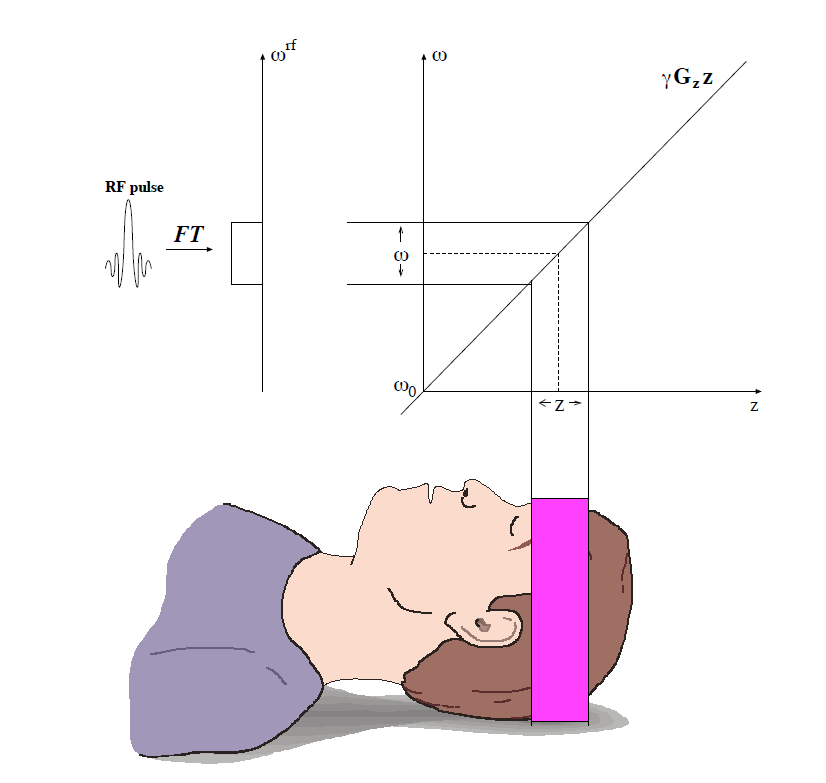
\includegraphics[width=1\textwidth,keepaspectratio]{sliceselect}
    \caption{Slice selection is shown in this image for a slice in the x-y plane. The slice select gradient ($G_z$) is applied along the z-axis. The RF pulse of frequency bandwidth $\Delta \omega$ will excite the protons precessing at this frequency range. Figure courtesy of \cite{Drobnjak07}}
    \label{fig:sliceselect}
\end{figure}

The second step is called \textit{spatial information encoding} and it is done after the RF pulse has excited a slice. Throughout the relaxation period, the Bloch equations will take the following form:

\begin{equation} \label{eq:258}
    \frac{dM_z}{dt} = \frac{M_0 - M_z}{T_1}
\end{equation}
\begin{equation} \label{eq:259}
    \frac{dM_x}{dt} = ( \omega_0 + \gamma \vec{G}(t) \cdot \vec{r} ) M_y - \frac{M_x}{T_2}
\end{equation}
\begin{equation} \label{eq:260}
    \frac{dM_x}{dt} = - (\omega_0 + \gamma \vec{G}(t) \cdot \vec{r}) M_x - \frac{M_y}{T_2}
\end{equation}

The solution for these equations will also include an accumulation in phase $\phi(\vec{r}, t) = - \int_0^t \omega(\vec{r}, t') dt' = -\omega_0 t - \gamma \int_0^t \vec{r} \cdot \vec{G}(t') dt'$. Thus, the solution in complex representation for the transverse magnetization will be:

\begin{equation}
    M_{+}(\vec{r},t) = \lvert M_{+}(\vec{r},0) \rvert e^{-t/T_2(\vec{r}) \, -i (\omega_0 t + \gamma \int_0^t \vec{r} \cdot \vec{G}(t') dt')}
\end{equation}

Considering the slice selection gradient being in the z direction, only x- and y-gradients are needed to encode spatial information in the selected slice. This information can be found in the spatial frequency of the detected signal:

\begin{equation}
    S(t) = \int \int 
            e^{-t/T_2(\vec{r})} M_{\perp}(\vec{r},0) 
                B_{\perp}(\vec{r}) 
                e^{ -i \gamma \int_0^t G_x(t')x + G_y(t')y dt'} dx dy
\end{equation}

This signal is collected during \textit{read out} as uniformly spaced time points \cite{Haacke1999} and stored in a matrix called the \textit{k-space}, where:
\begin{equation}
    k_x(t) = \frac{\gamma}{2 \pi} \int_0^t \vec{G}_x(t') dt' 
    \qquad\text{and}\qquad
    k_y(t) = \frac{\gamma}{2 \pi} \int_0^t \vec{G}_y(t') dt' 
\end{equation}
which, for constant gradients become:
\begin{equation}
    k_x(t) = \frac{\gamma}{2 \pi} G_x t
    \qquad\qquad\text{and}\qquad\qquad
    k_y(t) = \frac{\gamma}{2 \pi} G_y t
\end{equation}

Now, not taking into consideration the decay term $e^{-t/T_2(\vec{r})}$ during signal collection and using equation \ref{eq:225} to introduce the spin density of the sample, the signal in terms of k-space becomes:
\begin{equation}
    S(k_x, k_y) = \int \int \rho(x,y) e^{-i 2 \pi (k_x x + k_y y)} dx dy
\end{equation}

A visual representation of the k-space can be found in Figure~\ref{fig:kspace}. Note that k-space undergoes a Fourier transform in order to obtain the final image as seen in Figure~\ref{fig:reconstruction}.

Generally, k-space data is acquired line by line. Other techniques do exist, but they will not be discussed in this thesis. Every k-space line is a new repetition of the undergoing MRI sequence with a different phase-encoding step. This results in a total acquisition time ($T_A$) of:

\begin{equation}
    T_A = T_R \times N_{PE}
\end{equation}

where $T_R$ is the repetition time and $N_{PE}$ is the number of phase-encoding steps.

\begin{figure}[H]
    \centering
    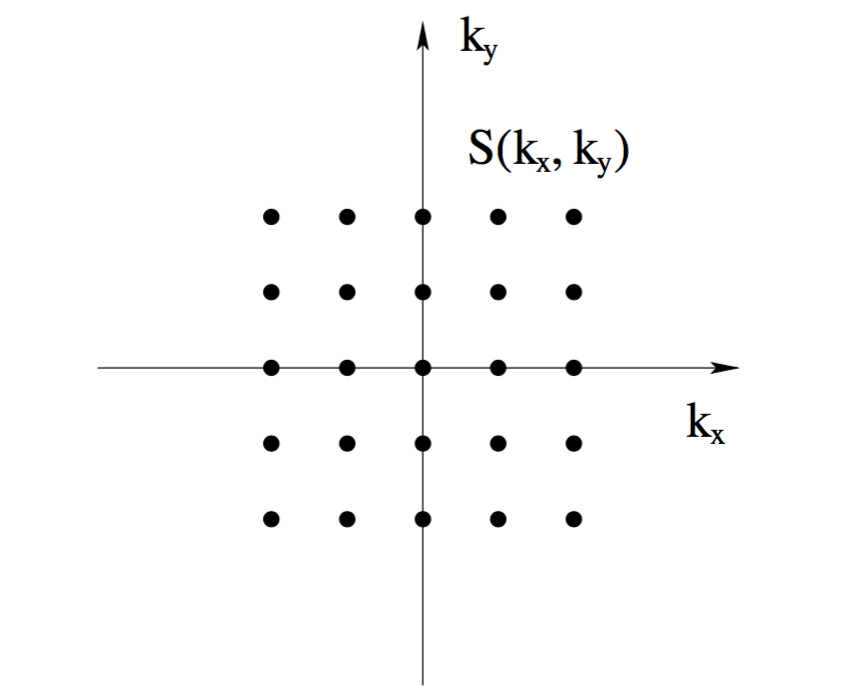
\includegraphics[width=.8\textwidth,keepaspectratio]{kspace}
    \caption{An example of a 4x4 k-space. Figure courtesy of \cite{Drobnjak07}}
    \label{fig:kspace}
\end{figure}

%%%%%%%%%%%%%
\subsection{Image Reconstruction}
We have seen so far how k-space is being constructed. The main steps are: first, by spatially varying the magnetic field and thus allowing for different frequencies and phases into spin's precessing behaviour, we encode spatial information into collections of spins. Second, the signal coming from the selected slice is sampled and a line of k-space is filled in with the corresponding Fourier coefficients. Third, the sequence is repeated with different phase-encoding steps until all lines of k-space are filled in. Once all the data has been collected, the Fourier transform is used to transform the k-space into an image (Figure~\ref{fig:reconstruction}). 

The distance between two adjacent points in k-space is called $\Delta k_x$ and $\Delta k_y$, depending on the direction (phase-encoding or frequency-encoding). These sampling intervals are inversely proportional to the image field-of-view (FOV) \cite{Deshmane2012}. This means that an increase in $\Delta k$ will lead to a decrease in the field-of-view in that direction. The highest spatial frequencies sampled in k-space are called $k_{x,max}$ and $k_{y,max}$ and they are inversely proportional to the resolution of the image (i.e. distance between consecutive points in the image: $\Delta x$ and $\Delta y$). Again, this means that by increasing $k_{x,max}$ or $k_{y,max}$ the distances will decrease and therefore the resolution of the final image will be higher. In conclusion, the final MR image characteristics are dependent upon the number of k-space points and the distance between them, all of which can be manipulated to obtain the desired image. 

\begin{figure}[ht]
    \centering
    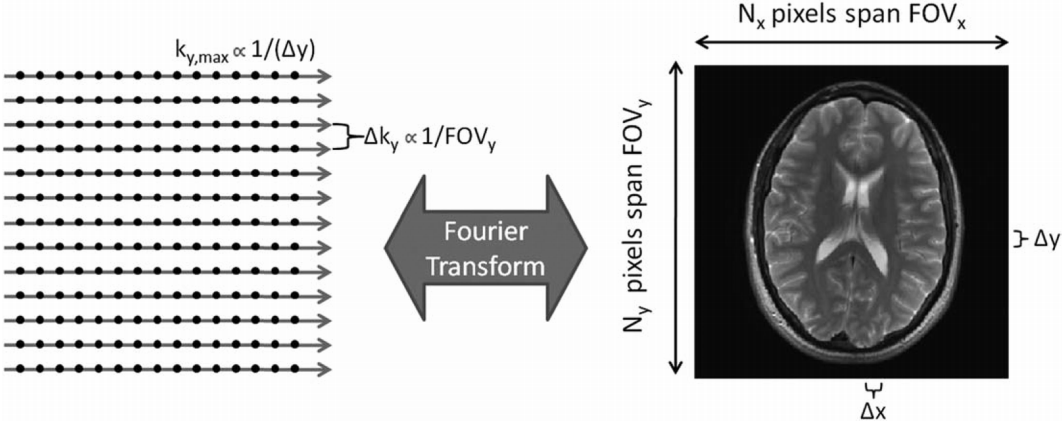
\includegraphics[width=1\textwidth,keepaspectratio]{reconstruction}
    \caption{A cartesian k-space undergoing a Fourier Transform to obtain the final image. Figure courtesy of \cite{Deshmane2012}}
    \label{fig:reconstruction}
\end{figure}

The main relationships discussed so far are presented in a mathematical form in equations \ref{eq:269}, \ref{eq:270}, \ref{eq:272} and \ref{eq:273}. The relationship between FOV and the sampling intervals are shown in the following two equations:

\begin{equation} \label{eq:269}
    FOV_x = \frac{1}{\Delta k_x} = \frac{1}{\frac{\gamma}{2 \pi} G_x \Delta t}
\end{equation}
and
\begin{equation} \label{eq:270}
    FOV_y = \frac{1}{\Delta k_y} = \frac{1}{\frac{\gamma}{2 \pi} \Delta G_y t_y}
\end{equation}

while the spatial resolution of the image is related to the highest spatial frequencies sampled in k-space by:

\begin{equation} \label{eq:272}
    \Delta x = \frac{1}{N_x \Delta k_x} = \frac{1}{2 k_{x,max}} = \frac{1}{\frac{\gamma}{2 \pi} G_x T}
\end{equation}
and
\begin{equation} \label{eq:273}
    \Delta y = \frac{1}{N_y \Delta k_y} = \frac{1}{2 k_{y,max}} = \frac{1}{\frac{\gamma}{2 \pi} 2 G_{y,max} t_y}
\end{equation}

A more interesting discussion arises when k-space data are missing. This can happen if the sampling rate is not high enough (at least twice as fast as the highest frequency component contained within the MRI signal) to reconstruct the signal. This is called the \textit{Nyquist-Shannon} theorem and if it is broken an interesting artefact occurs called \textit{aliasing} \cite{Deshmane2012}. A nice depiction of this phenomenon can be seen in Figure~\ref{fig:partialkspace} where the rightmost column shows what happens when undersampling occurs in the phase-encoding direction.

\begin{figure}[ht]
    \centering
    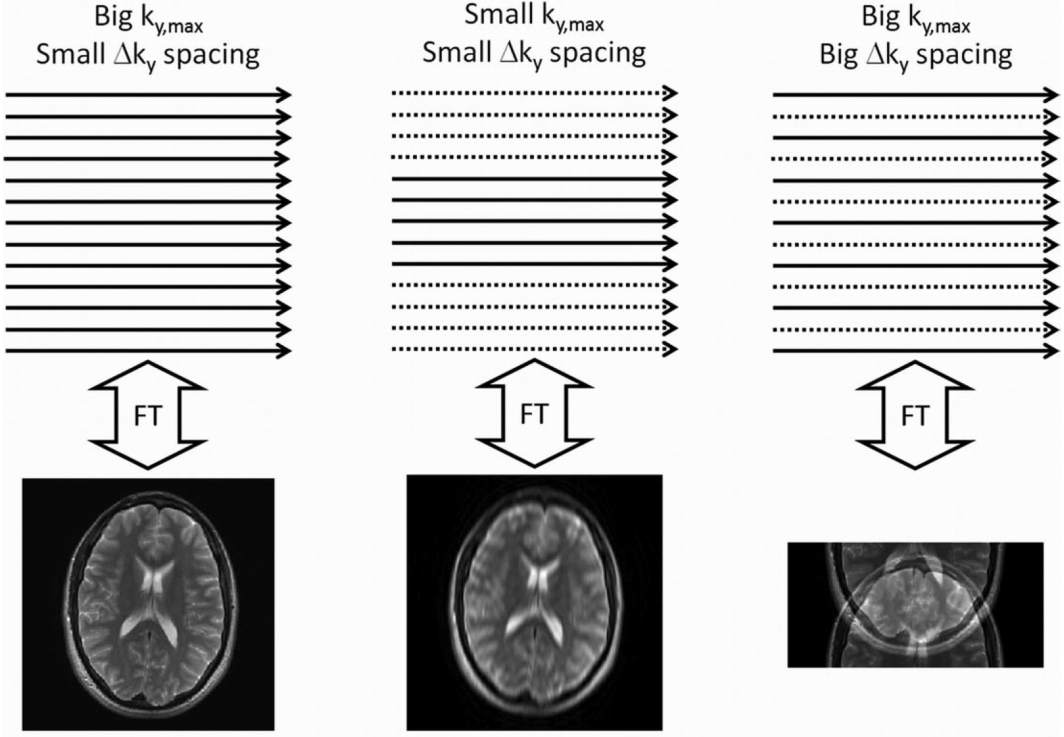
\includegraphics[width=1\textwidth,keepaspectratio]{partialkspace}
    \caption{The left column shows a fully sampled k-space which will yield a high-resolution image. The middle column shows what happens to the final image when higher frequencies are discarded ($k_{y,max}$ is decreased). This will yield a lower resolution image, but keep the same FOV. The last column shown an aliased image example which happened because $\Delta k_y$ was increased while $k_{y,max}$ was kept constant. Figure courtesy of \cite{Deshmane2012}}
    \label{fig:partialkspace}
\end{figure}

Mathematically, this can be explained with the following deduction. We start from the relationship between $\Delta k$ and FOV for the case shown in the left side of Figure~\ref{fig:partialkspace}: $\Delta k_y = \frac{1}{FOV_y}$. By missing every other line of k-space we basically increase the spacing twofold. Therefore, let's consider this new relationship as $\Delta k_y' = \frac{1}{FOV_y'}$. But, we also know that:

\begin{flalign*}
    \Delta k_y' = 2 \Delta k_y = \frac{2}{FOV_y} = \frac{1}{\frac{FOV_y}{2}} = \frac{1}{FOV_y'}
\end{flalign*}

Therefore, our new field-of-view is half of the previous one $FOV_y' = \frac{FOV_y}{2}$. This leads to aliasing as the missing FOV folds itself on top of the halved one. This theoretical consideration is important to remember for the next section where Parallel Imaging techniques are introduced as a means of reducing the amount of time a scan requires by reducing the number of phase-encoding steps and resolving the aliasing that inevitably happens.

%%%%%%%%%%%%%%%%%%%%%%%%%%
\section{Parallel Imaging}

%%%%%%%%%%%%%
\subsection{Motivation}
We have discussed so far about the basic steps needed to acquire MR images, from the physics of spins precessing in magnetic fields to image reconstruction from k-space data. However, one topic that has not been fully addressed was the imaging time. Indeed, an MRI scan is a procedure that can take from a few minutes to a few hours depending on the characteristics of the resulting images. As can be expected, a way to reduce the scan time is a nice to have requirement for both patient comfort and reduced movement artefacts. 

For this reason, in the late 1980s, fast imaging sequences such as \textit{Echo Planar Imaging (EPI)} or \textit{Fast Low-Angle Shot (FLASH)} were invented. Both FLASH \cite{Haase1986} and EPI \cite{DeLaPaz1994} manage to reduce the imaging time per slice to a few tens of milliseconds which leads to imaging full volumes in a couple of seconds and limit the possibility of movement during acquisition. However, pushing the imaging time even further down becomes problematic as the hardware components face technical limitations when it comes to rapidly switching on and off the gradients. Also, patient safety is at risk when gradient strengths and slew rates exceed certain thresholds. 

Under these circumstances, new techniques had to be implemented to overcome these limitations. This is how \textit{parallel acquisition techniques} came into being. These are not new imaging sequences, but they are a collection of reconstruction algorithms that can be applied to almost all existing imaging sequences without changing the scanner's hardware behaviour.  

Actually, the main idea behind \textit{Parallel MRI (pMRI)} is to replace phase-encoding steps from k-space data with rf coil information. The coil data comes from a collection of receivers working in parallel (simultaneously). Their spatial sensitivity profiles can be used to undersample k-space, which translates into skipping some time-consuming phase-encoding steps. As a result, the acquisition time is reduced by a so called \textit{acceleration factor R}, while the reconstruction algorithms take the time-consuming burden. 

Undoubtedly, there are many advantages that parallel imaging techniques bring. Some of them are worth mentioning:
\begin{itemize}
    \item Real-time imaging
    \item Less artifacts caused by movement
    \item Shorter periods for holding one's breath
    \item Less contrast agent in MR angiographies
\end{itemize}

All in all, pMRI is widely used in clinics nowadays and so a closer look at how they work and on what principles they are based upon is worthwhile. This will be the subject of the next subsections where basic concepts are presented and one of the algorithms is presented in more depth.

%%%%%%%%%%%%%
\subsection{Basic Concepts}
Parallel Imaging is used in MRI in order to reduce scanning time. This is possible because time-consuming phase-encoding steps are skipped during the scan. Unfortunately, this means that the final images will be aliased. The purpose of pMRI techniques is, therefore, to resolve the 'folding' and to provide clinicians with good data sets. Currently, there are a few approaches to this issue, but before mentioning them it is worth discussing about what they all have in common:

\begin{enumerate}

    \item For all available techniques k-space data are undersampled in the phase-encoding direction. As a result, the definition of the acceleration factor is $R = \frac{\text{number of lines for a fully sampled k-space}}{\text{number of lines for the undersampled k-space}}$ \cite{Deshmane2012}. For example, skipping every other line of k-space results in an acceleration factor $R = 2$.
    
    \item Imaging is done using an array of coils whose sensitivity profiles are acquired during a prescan at the beginning of the MRI examination. Because the coils do not have a homogeneous sensitivity map, but they are rather more sensitive to the signal originating from the tissue mass which is located more closely to the coil, they add an extra source of spatial information for the reconstruction step.
    
    \item An algorithm reconstructs the final unaliased, full FOV image by using the undersampled data and the individual coil sensitivities.
    
\end{enumerate}

\begin{figure}[ht]
    \centering
    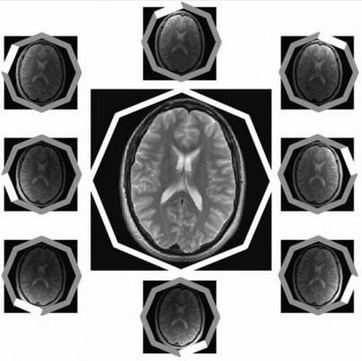
\includegraphics[width=.7\textwidth,keepaspectratio]{coils}
    \caption{This image shows an example of an 8-channel array, with the coils distributed around the object of interest. Figure courtesy of \cite{Deshmane2012}}
    \label{fig:coils}
\end{figure}

As it is evident by now, in pMRI techniques an important actor is the coil. This piece of hardware is more commonly known as \textit{the multichannel receiver array} as it is made up of a series of receiver coils which are uniformly distributed around the organ of interest. Any of the individual channels are more sensitive to the signal coming from an area closer to it and less sensitive as the distance increases.

Clinically, the multicoil receiver array contains from 4 to more than 32 channels that have their own associated sensitivity profiles. They can be arranged either linearly as it happens for spine MR imaging, or radially as it is more common for neuroimaging. An example of how 8 coils could be circularly placed is seen in Figure~\ref{fig:coils}. As the reconstruction algorithm relies on extra information brought by the coils' sensitivity maps, i.e. the sensitivity differences that exist between coils, the acceleration can only take place in the direction of the receiver array. This means that, in practice, there is a lot of thought put behind the placement of these channels such that the final configuration provides the maximum possible acceleration in the phase-encoding direction. Moreover, any overlap between the sensitivity profiles is avoided as much as possible.

\begin{figure}[ht]
    \centering
    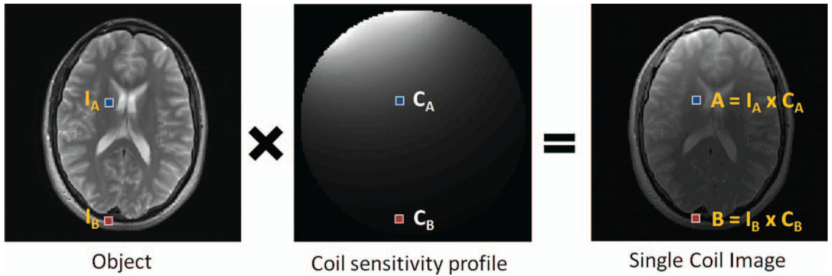
\includegraphics[width=\textwidth,keepaspectratio]{onecoilsens}
    \caption{A single coil image is obtained by 'weighting' the coil sensitivity profile with the object image. Figure courtesy of \cite{Deshmane2012}}
    \label{fig:onecoilsens}
\end{figure}

Turning to an individual coil, an MR image which could possibly result is shown in Figure~\ref{fig:onecoilsens}. The mathematical interpretation of how the final image looks when the signal was collected by a receiver coil which has an associated sensitivity map (as shown in the middle image) is that every voxel in the final image will be 'weighted' by the corresponding sensitivity index. As such, the 2 locations, A and B, from the final MR image can be thought of as having intensity values which result from multiplying the coil sensitivity at location A with the actual intensity of the given object if the coil used was a homogeneous one:

\begin{equation}
    A = C_A \times I_A \text{ and } B = C_B \times I_B
\end{equation}

Consequently, an acceleration of scan time can be achieved if each individual coil only collects a smaller FOV which is also closer to itself. This is the basis for a very simple parallel imaging reconstruction algorithm called PILS (\textit{Partially parallel imaging with localized sensitivities} \cite{Griswold2000}) which simply puts together the images generated by each coil. An example with 2 coils can be seen in Figure~\ref{fig:pils}.

\begin{figure}[ht]
    \centering
    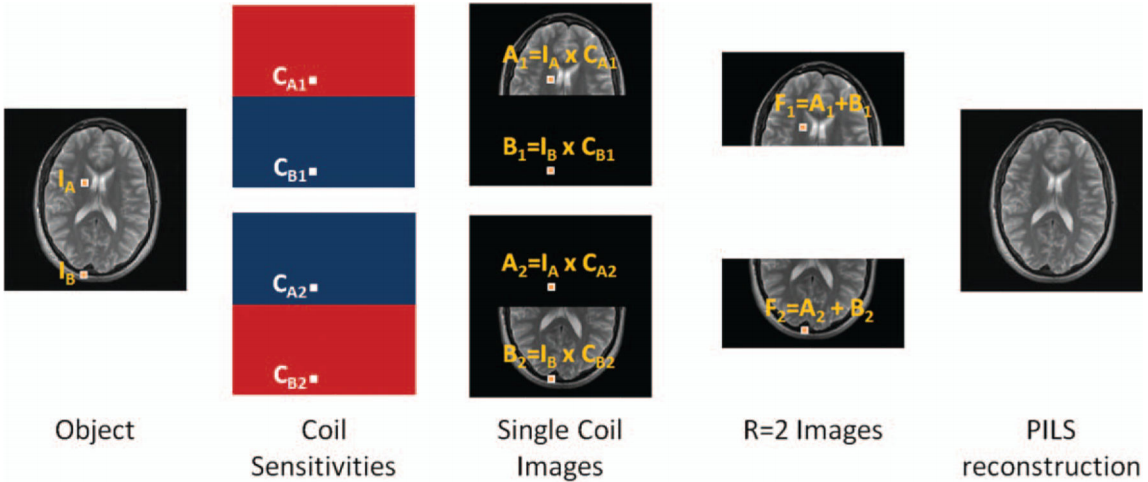
\includegraphics[width=\textwidth,keepaspectratio]{pils}
    \caption{An example of a parallel imaging technique performed with a 2 channel array where the coils have non-overlapping sensitivity profiles. Figure courtesy of \cite{Deshmane2012}}
    \label{fig:pils}
\end{figure}

Obviously, in practical terms this is not feasible. Coil sensitivities will overlap and an algorithm like PILS will fail to reconstruct the image. A more powerful algorithm which unfolds the aliased images, reconstructs a full FOV final image, uses overlapping sensitivity profiles and is actually widely used clinically called SENSE will be the subject of our discussion in the following subsection.

%%%%%%%%%%%%%
\subsection{SENSE Reconstruction} \label{sect:senserec}
Sensitivity Encoding for Fast MRI, or SENSE, is a parallel imaging reconstruction algorithm which is widely used in the clinics. It relies on knowledge of the sensitivity profiles of the individual coils which are used to receive the signal. In practice, the coil maps are calculated at the beginning of a sequence during a prescan. This section is concerned with the main concepts that form the basis for SENSE reconstructions. Although not without problems, mainly caused by patient movement during scan time, SENSE is one of the most popular algorithms used in clinics today. 

As we have discussed before, all parallel imaging techniques have a few things in common. First, undersampled k-space data is acquired and this results in aliased images. If an acceleration factor $R = 2$ is used, then the folding that occurs will translate into 2 pixels being on top of each other. An example of how this might look for 4 channels is presented in Figure~\ref{fig:sense}.

\begin{figure}[ht]
    \centering
    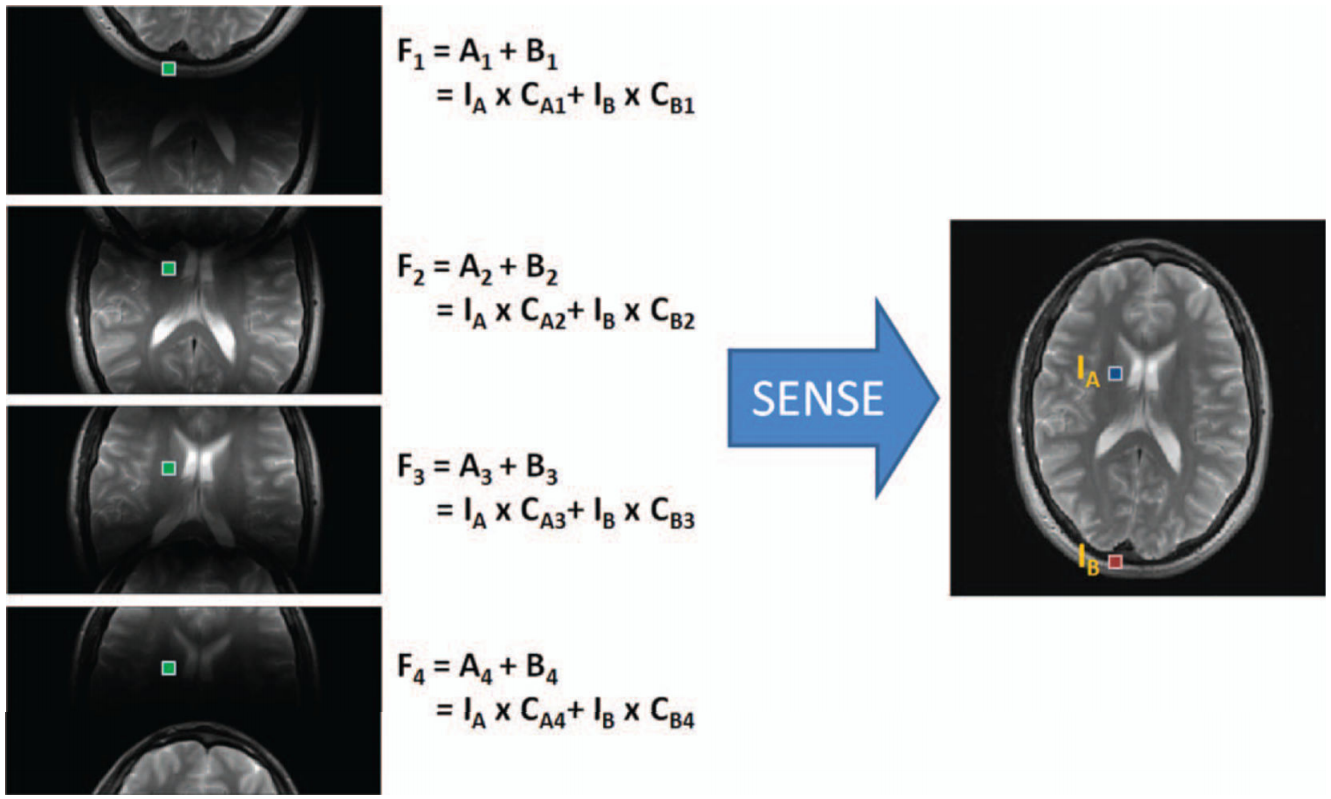
\includegraphics[width=1\textwidth,keepaspectratio]{sense}
    \caption{A 4 channel array SENSE reconstruction for an acceleration factor $R = 2$ is shown here as example. Figure courtesy of \cite{Deshmane2012}}
    \label{fig:sense}
\end{figure}

As mentioned before, SENSE relies on the sensitivity profiles of the coils. It uses this information and the aliased images to 'unfold' the image. This works because, as can be seen in Figure~\ref{fig:sense} where $R = 2$, every voxel intensity is a juxtaposition of 2 intensity values that are coming from the 2 spatial locations which are now on top of each other. So, for example, at the coordinate shown in the first image from the figure, the intensity from the aliased image is just the sum of intensities of those 2 spatial locations ($A_1$ and $B_1$). Moreover, these two locations are actually, as was shown in Figure~\ref{fig:onecoilsens}, directly related to the sensitivity value of the coil at that position. Now, using the same approach for all voxels found at the same spatial coordinate in all images and using the coil sensitivity profiles, we form a linear system that can be solved mathematically.

In our example, the four equations (one for each coil) are:

\begin{flalign*}
    F_1 & = A_1 + B_1 = I_A \times C_{A1} + I_B \times C_{B1} \\
    F_2 & = A_2 + B_2 = I_A \times C_{A2} + I_B \times C_{B2} \\
    F_3 & = A_3 + B_3 = I_A \times C_{A3} + I_B \times C_{B3} \\
    F_4 & = A_4 + B_4 = I_A \times C_{A4} + I_B \times C_{B4} 
\end{flalign*}

which, in matrix form is:

\begin{flalign*}
    \left[
    \begin{array}{c}
        F_1 \\
        F_2 \\
        F_3 \\
        F_4
    \end{array}
    \right]
    = 
    \left[
    \begin{array}{c c }
        C_{A1} & C_{B1} \\
        C_{A2} & C_{B2} \\
        C_{A3} & C_{B3} \\
        C_{A4} & C_{B4} 
    \end{array}
    \right] 
    \times
    \left[
    \begin{array}{c}
        I_A \\
        I_B
    \end{array}
    \right] 
    \Rightarrow
    F = C I
\end{flalign*}

By using Moore-Penrose pseudoinverse, the system of equations can be solved to find the underlying intensity values of the 2 locations, A and B:
\begin{flalign*}
    I = (C^T C)^{-1} C^T F = C^\dagger F
\end{flalign*}
This operation is applied for every spatial location in the image.

As can be expected, a few requirements are needed in order to be able to solve the system of equations. First of all, the number of coils has to be higher than the number of pixels which are juxtaposed for the reconstruction to work. Second, independent channels must not fully intersect each others' sensitivity profiles in order to allow for different weightings of the folded signals. Finally, parallel imaging is known to cause lower signal-to-noise ratio (SNR) values than non-parallel imaging methods due to k-space undersampling \cite{Aggarwal2003}\cite{Xu2005} and coil design \cite{Weiger2001}\cite{Zhu2004}\cite{Ohliger2003}\cite{Lee2004}. The signal-to-noise ratio for SENSE is calculated with the following formula:
\begin{equation}
    SNR_{SENSE} = \frac{SNR_{Original}}{g \sqrt{R}}
\end{equation}
where $g$ is defined as the geometry factor of the coil, or \textit{g-factor} and $SNR_{Original}$ is the signal-to-noise ratio of an MRI image when pMRI is not performed. The "g-factor" describes how good the multichannel receiver array encodes the magnetization distribution of the object \cite{Omer2010}. It is a measure which indicates how much a coil array magnifies the noise at a given location and it is dependent on the number of aliased replicates.

In mathematical terms, the \textit{g-factor} at location $y$ is defined as:
\begin{equation}
    g_y = \sqrt{ [(C^T \Psi^{-1} C )^{-1}]_{yy} (C^T \Psi^{-1} C )_{yy} }
\end{equation}
where $\Psi$ is the noise correlation matrix and $C$ is the sensitivity encoding matrix. This concept is highly used in parallel imaging techniques as it enforces the physical arrangement of the coils used in pMRI scans.

In summary, this section has described the most important concepts behind parallel imaging techniques and reconstructions, with a focus on one of the most popular algorithms, SENSE. The main disadvantage of SENSE reconstruction is the need for accurate coil sensitivity profiles. In addition, motion can be a determining factor when it comes to image quality. Despite these difficulties, SENSE is widely used clinically in order to accelerate MRI scans.





